\chapter{Network Architecture}
\label{ch:architecture}
\pagestyle{headings}

As shown in the figure \ref{fig:tarnet}, our targeted network is a mixed section requiring the use of Exterior Gateway Protocols (IGP) and Internal Gateway Protocols (EGP) in order be able to share routes routes between the two BGP ends (named \textit{E} and \textit{F}) going through a BMX6 Mesh Network (from report \cite{bgpbmx6} - in Catalan). 

As shown in the figure:
\begin{itemize}
    \item \textbf{Infrastructure Super Node 1} (ISN1): BGP Supernode connected to the BGP network (Guifi.net, section 1) via wireless and to the MXN1 Router through Ethernet.     
    \item \textbf{Mesh eXchange Node 1} (MXN1): LEDE/OpenWRT router connected via Ethernet to the ISN1 and to the antenna (or an Ethernet port) providing access to the Mesh Network. This frontier node provides BGP to BMX6 route-sharing capabilities using Bird Daemon.
    \item \textbf{Mesh Network}: A number of Nodes connected using BMX6 forming an isle between BGP nodes.
    \item \textbf{Mesh eXchange Node 2} (MXN2): LEDE/OpenWRT router connected via Ethernet to the ISN2 and to the antenna (or an Ethernet port) providing access to the Mesh Network. This frontier node provides BGP to BMX6 route-sharing capabilities using Bird Daemon.
    \item \textbf{Infrastructure Super Node 2} (ISN1): BGP Supernode connected to the BGP network (Guifi.net, section 2) via wireless and to the MXN2 Router through Ethernet.
\end{itemize}

\newpage

\section{Routing requirements}
Routing requirements to successfully ensure that all routes are shared between both BGP ends are:

\begin{itemize}
    \item Routes must be shared/announced between ISN1 (\textbf{E}) and ISN2 (\textbf{F}).
    \item Mesh Network's Routes (BMX6 - \textbf{C}\&\textbf{D}) must be shared/announced to ISN1 and ISN2 (\textbf{A}\&\textbf{B}). Therefore, shared/announced to Guifi.net network.
    \item ISN1 and ISN2 Routes (BGP - \textbf{A}\&\textbf{B}) must be shared/announced to the Mesh Network (\textbf{C}\&\textbf{D}).
    \item MXN1/2 must configure Bird to use a custom Routing Table that will be shared with BMX6.
    \item MXN1/2 must configure BMX6 to use the \textit{Table} plugin in order to redirect its routes from Kernel's Table to a custom one.
    \item MXN1/2 must configure Bird to set them both as BGP Peers to stablish an iBGP session between them (AS2).
    \item MXN1 must configure Bird to set ISN1 as BGP Peer AS1
    \item MXN2 must configure Bird to set ISN1 as BGP Peer AS3
\end{itemize}

\subsection{Caveats}
There is an important caveat with this network distribution:

Current version of BMX6 is not able to handle the number of routes that this Guifi.net BGP section is sharing (2.500+). Therefore, BMX6 starts aggregating routes, which eventually shut-downs the service and leaves the node overloaded as it is not able to achieve it.

In order to avoid this disruptive issue, Bird Daemon filter scripting capabilities available in MXN1 and MXN2 allow to reduce the geographical scope of the routes imported and exported to/from the Barcelon\`{e}s\footnote{\href{https://guifi.net/barcelones}{Barcelon\`{e}s}: Network Zone including Badalona, Barcelona, Hospitalet del Llobregat, Sant Adri\`{a} del Besos and Santa Coloma de Gramanet} Zone.

\begin{landscape}

\begin{figure}[ht!]
        \centering
        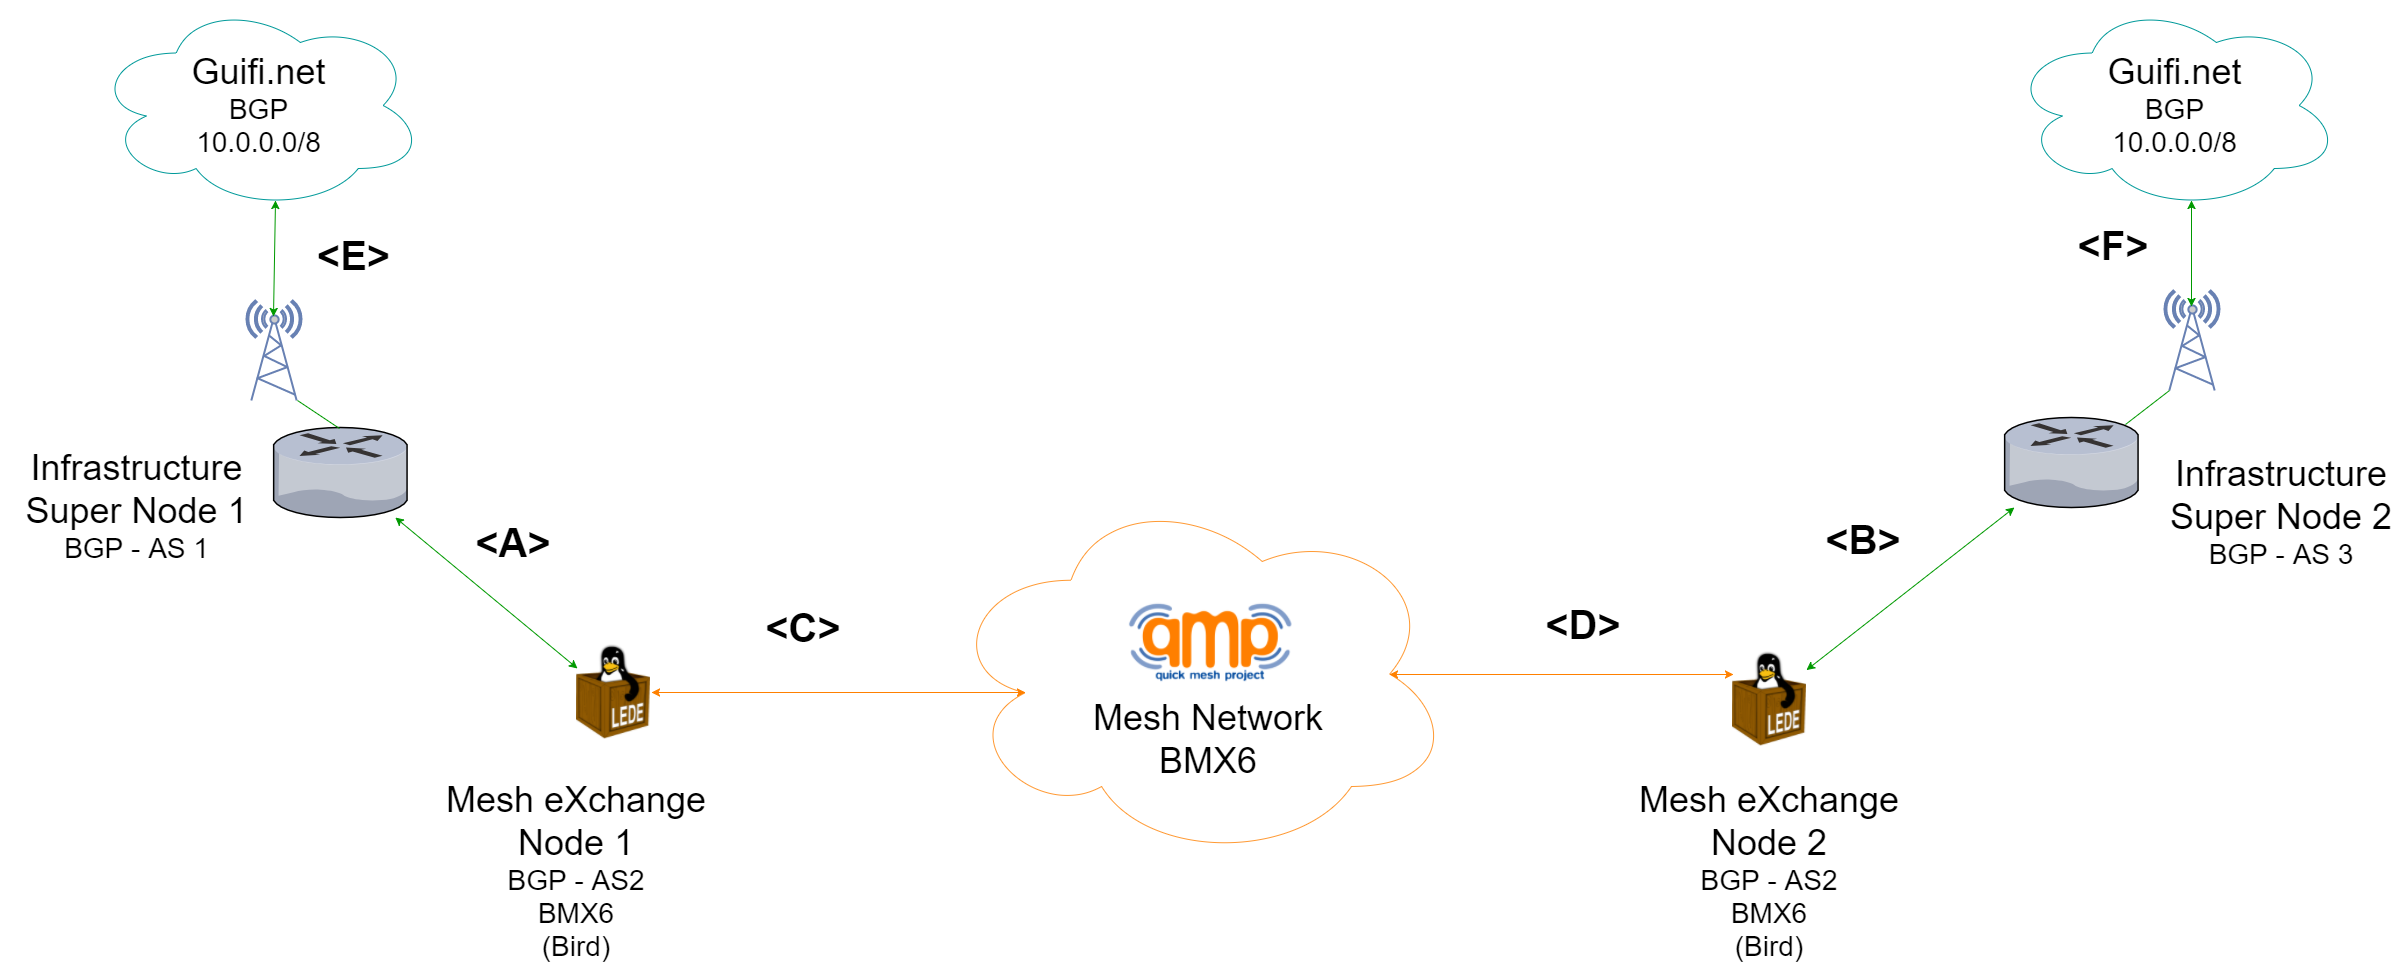
\includegraphics[width=\hsize]{images/targetnet}
        \caption{Production Network targeted in this project}
        \label{fig:tarnet}
	\end{figure}
\end{landscape}
\newpage

\section{Real environment testing}
Although it has not been possible to test Package's improvements due to the impact that a change like this could incur in a live network involving several critical \textit{Super Nodes} and all the routes in the Mesh Network, it is foreseen to be updated soon in a planned and backed up manner.

\subsection{Development environment testing}
The \textit{Universitat Oberta de Catalunya} and V\'{i}ctor have provided me a number of Virtual Machines plus a number of network resources in order to simulate our target network but without the risk of damaging the production network or flooding unwanted routes to Guifi.net.

\begin{itemize}
    \item VPN access to the Guifi Network using UOC's resources.
    \item 4 Virtual Machines using LEDE17.01 Firmware.
    \item Virtual Bridge to connect the VMs simulating a Mesh Network.
    \item Network way through two different network sections.
    \begin{itemize}
        \item Connection using UOC's Super Node
        \item Virtual Machine 4 connects through UPF\footnote{Universitat Pompeu Fabra}'s internal network to find path out to a near Guifi network.
    \end{itemize}
\end{itemize}

\begin{landscape}

\begin{figure}[ht!]
        \centering
        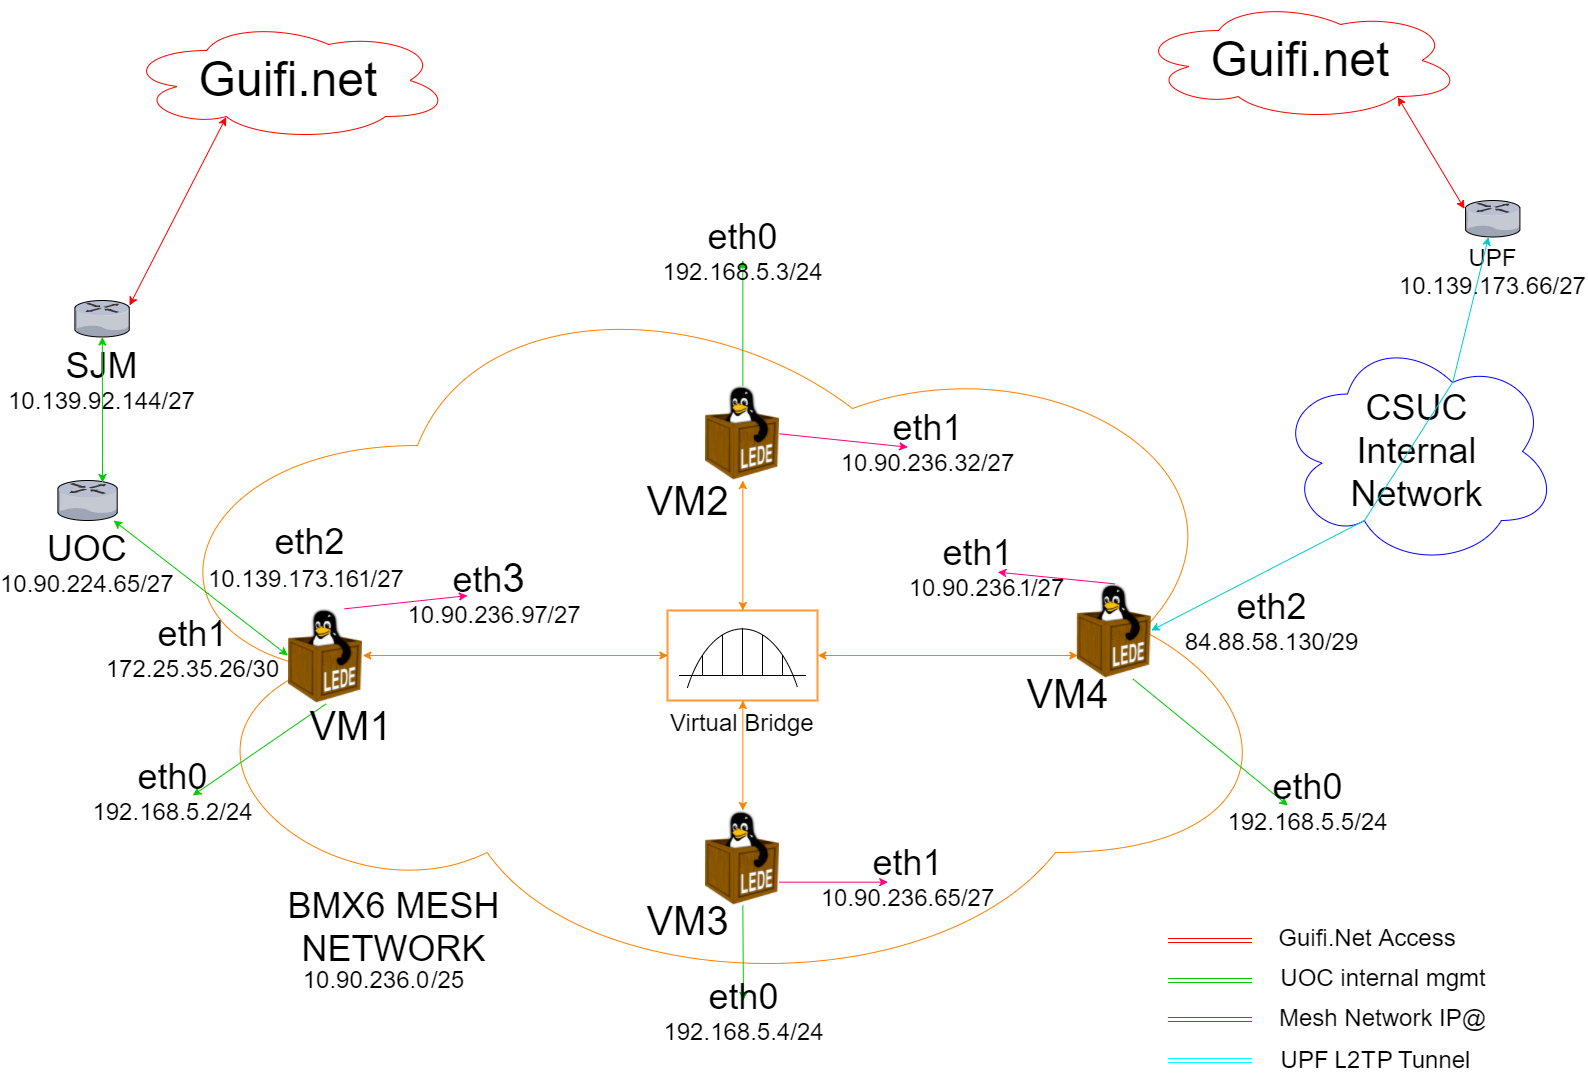
\includegraphics[width=\hsize]{images/devnetfull}
        \caption{Development Network simulating production's environment}
        \label{fig:devnet}
	\end{figure}
\end{landscape}
\newpage

